\chapter{Higgs 粒子的探测}

\section{Higgs 粒子的三个主要衰变道}

在 ATLAS 中,最主要的衰变道就是四轻子衰变道。它先由希格斯粒子衰变成两个 $Z$ 玻色子,再衰变成四个轻子,这里的轻子是电子和 $\mu$ 子。在寻找的过程中,要寻找两对单独的轻子对,每对轻子对有相同的味道和相反的电荷。其中,候选的 $\mu$ 子由 $\mu$ 子探测器重构,电子则有电磁量能器重构,且由单轻子或双轻子判选系统来区分动量。每一个电子的横向动量要大于 \qty{7}{GeV},而 $\mu$ 子则要大于 \qty{6}{GeV},且 \emph{赝快度 (Pseudorapidity)} $|\eta|$ 要分别在 $2.47$ 和 $2.7$ 内。同样,对轻子之间的距离也有要求,对于相同味道的轻子,要满足 $\Delta R$ 大于 $0.1$,其它的则要求大于 $0.2$。所产生的四个轻子,也就是两对轻子对,会根据其不变质量再进行划分。与 $Z$ 玻色子质量最接近那对轻子被称为首要轻子对,另一对则是次要轻子对。根据它们的味道,衰变道还要再分为四个子衰变道,分别是 $4$ 个电子、双电子双 $\mu$ 子、双 $\mu$ 子双电子和四个 $\mu$ 子。这些子衰变道的本底率和质量分辨是不一致的,因此对希格斯粒子寻找的灵敏度也不同,要分开分析,最后再和在一起。对于四 $\mu$ 子信号重构与选择效率,\qty{7}{TeV} 下是 $37\%$,\qty{8}{TeV} 下是 $36\%$;双电子双 $\mu$ 子和双 $\mu$ 子双电子在这两个能量下分别为 $20\%$和 $22\%$,而 $4$ 轻子则是 $15\%$ 和 $20\%$

在这个衰变道中,主要本底源于 $Z$ 玻色子、$Z$ 玻色子加上 \emph{喷注 (jet)} 与正反 $t$ 夸克。这些噪音会用蒙特卡罗模拟和具体数据来进行预测。而且还与次要轻子对的味道有关,所以还要分成 $\mu$ 子对和电子对的情况来分别处理。

最后的结果如图所示,这是四轻子不变质量的分布图,背景的红色和紫色部分是预测的本底,蓝色则是预测的希格斯粒子信号。可以看出,在 \qty{125}{GeV} 左右,确实有目标信号的存在。

\begin{figure}[htbp]
    \centering
    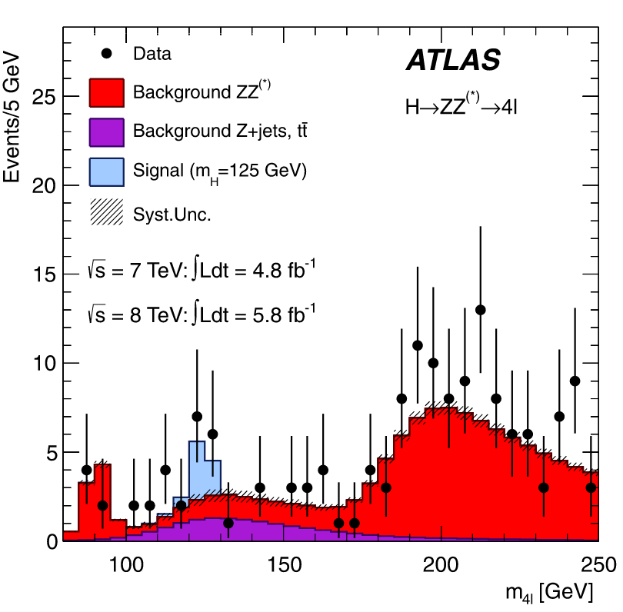
\includegraphics[width=0.6\textwidth]{pic/events.png}
    \caption{Signal at \qty{125}{GeV}.}
    \label{fig:events}
\end{figure}

另一个重要的衰变道是双光子衰变道。相对于其他夸克或胶子等强子对末态,双光子的分支比要小得多,但更容易识别。它的数据是则是由双光子触发判选系统选择的,并且需要在电磁量能器中形成两束光子簇的能量。在能量为 \qty{7}{TeV} 时,每个光子簇的横向能量要大于 \qty{20}{GeV};\qty{8}{TeV} 时,则要分别大于 \qty{35}{GeV} 和 \qty{25}{GeV}。并且由于存在能量损失和能量渗漏,要用蒙特卡罗模拟来修正候选光子的能量。双光子的不变质量则由电磁量能器中测的光子能量、光子在量能器中的方位角 $\phi$ 和初始顶点与碰撞点计算出的赝快度η得出。最终 在 \qty{100}{GeV} 到 \qty{160}{GeV} 的不变质量范围内,在能量为 \qty{7}{TeV} 和 \qty{8}{TeV} 时,分别选出了 $23788$ 和 $35251$ 对候选的双光子。为了提高对希格斯粒子寻找的灵敏度,还将这些事例分成了 $10$ 个种类。这是划分出的种类和对应的事例数量。这里的 $p_{Tt}$ 是双光子横向动量垂直于轴的分量。

\begin{figure}[htbp]
    \centering
    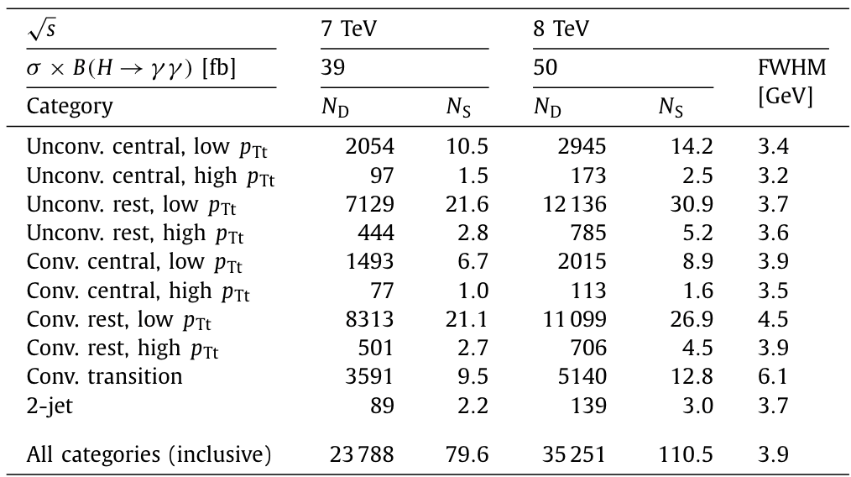
\includegraphics[width=0.6\textwidth]{pic/10.png}
    \caption{$10$ 种事例}
    \label{fig:10}
\end{figure}

双光子衰变道中,主要的本底是标准模型下,高能质子和质子对撞产生的双光子末态,同时还有产生的喷注被误认为光子,以及 Drell-Yan 过程的影响,这是一个产生于高能强子散射的过程。在双光子衰变道的本底预测中,按之前分的不同种类用了不同的处理手段。比如说对某些种类,则用四阶伯氏多项式去预测,而其他的则用指数函数去处理。

最后的结果如图所示,上面的这张红色的,虚线是相对希格斯粒子质量为 \qty{126.5}{GeV} 预测的本底,实线是本底加上希格斯粒子的信号。下面蓝色的则是加权后的情况,这里是将不同种类的数据进行了不同权重的处理。这两个则是将本底扣除的结果。也是能从双光子的不变质量谱上发现一个峰。

\begin{figure}[htbp]
    \centering
    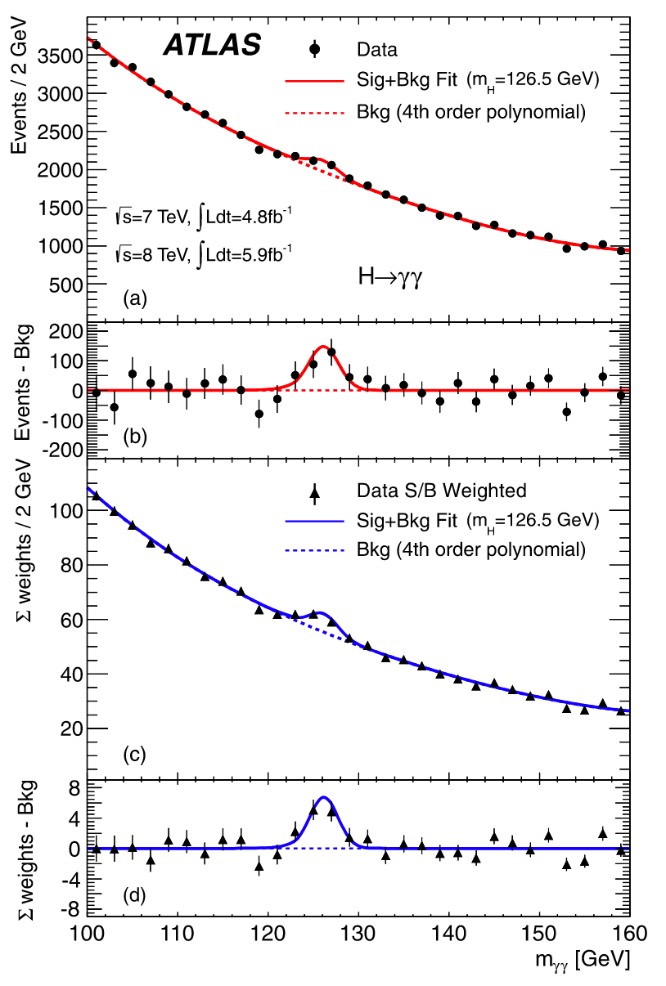
\includegraphics[width=0.6\textwidth]{pic/atlas.png}
    \caption{ATLAS 实验结果}
    \label{fig:ATLAS}
\end{figure}

\section{ss}

通过引入一个信号强度参数 $\mu$,建立模型 $\mu s(m) + b$;

假设检验问题:

\begin{itemize}
    \item 零假设 $H_0: \mu=0$,表示没有信号,只有背景存在;
    \item 备择假设 $\mu > 0$,表示存在一个信号。
\end{itemize}

我们想要检验的是是否存在一个信号强度大于 $0$ 的共振。

模型中的背景分布 $b$ 和信号分布 $s$ 可能还依赖于其他干扰参数,但在这里的表示中被省略了。质量 $m$ 是另一个干扰参数,但在零假设下不存在,因为背景分布 $b$ 不依赖于 $m$。因此,这个检验问题中存在一个只在备择假设下出现的干扰参数。

当搜索范围内可能存在共振时,我们会寻找超过背景的最大事件过剩。具体来说,如果 $q(m)$ 是针对固定质量的检验统计量,并且较大的 $q(m)$ 值表示与零假设的兼容性降低,那么整个范围的检验统计量将是 $q(\hat{m})=\max_m ⁡[q(m)]$,即取所有固定质量下的检验统计量的最大值。

实验中,我们感兴趣的参数是 \emph{全局信号强度因子 (Global signal strength factor)}$\mu$ \footnote{使用基于轮廓似然比的统计量 $\lambda_\mu$ 来测试 $\mu$ 的假设值。该测试统计量从对数据进行的完整似然拟合中提取了信号强度的信息。似然函数包括描述系统误差及其相关性的所有参数。},它作为一个比例因子影响了标准模型中预测的希格斯玻色子信号的总事件数。

排除限制是基于 CLs 方法 \footnote{Confidence Level as a function of the test Statistic} 进行的;当 CLs 小于 $5\%$ 时,我们将 $\mu$ 值视为在 $95\%$ 的置信水平下被排除。当在质量为 $m_H$ 的情况下排除 $\mu=1$ 时,我们认为质量为 $m_H$ 的标准模型希格斯玻色子已经被排除,置信水平为 $95\%$。

对于在给定搜索区域中观测到最显著过剩的全局概率,计算全局概率与局部概率之比——试验因子 (trial factor),用于纠正“look elsewhere effect” \footnote{"Look elsewhere effect"是指在进行多次统计假设检验时可能出现的误导性结果。当进行多个假设检验时,有一定概率会出现某个检验结果达到显著性水平,即使在没有真实效应的情况下也可能发生。}。 统计检验是以假设的希格斯玻色子质量 $m_H$ 的值为步长进行的。

相关系统误差的主要来源如下:

\begin{enumerate}
    \item 累计亮度:累计亮度的不确定性在通道之间被视为完全相关。
        \begin{itemize}
            \item 对于 \qty{7}{TeV} 的数据,它为 $3.9\%$
            \item \qty{8}{TeV} 的数据的不确定性为 $3.6\%$。
        \end{itemize}
    \item 电子和光子触发识别:电子和光子触发和识别效率的不确定性在电子和光子之间被视为完全相关。
    \item 电子和光子能量标度:$H \to ZZ(*) \to 4\ell$ 和 $H\to\gamma\gamma$ 通道中的电子和光子能量标度由五个参数描述,它们详细说明了系统误差的来源。
    \item $\mu$ 子重建:影响 $\mu$ 子的不确定性被分为与内部探测器 (ID) 和磁谱仪 (MS) 相关的部分,以便更好地描述使用不同的 $\mu$ 子鉴别标准和正负电子动量范围的通道之间的相关效应。
    \item 喷注能量刻度和缺失横向能量:喷注能量刻度和喷注能量分辨受到与喷注的 $p_T$、和味有关的不确定性的影响。结果对于关于这些不确定性来源之间相关性的各种假设的敏感性被发现是可忽略的。除了 JES 不确定性外,还包括了一个与未重建的物理对象不相关的低能喷注活动有关的 $E_T^miss$ 不确定性分量。
    \item 理论不确定性:相关的理论不确定性主要影响信号预测。
\end{enumerate}

使用 \qty{8}{TeV} 数据对于 $H\to ZZ(*)\to 4\ell$、$H\to\gamma\gamma$、$H\to WW(*)\to e\nu\mu\nu$ 通道的分析,以及对 \qty{7}{TeV} 数据在前两个通道中的改进,相较于先前的综合搜索,在低质量区域带来了显著的灵敏度提升。

\begin{figure}[htbp]
    \centering
    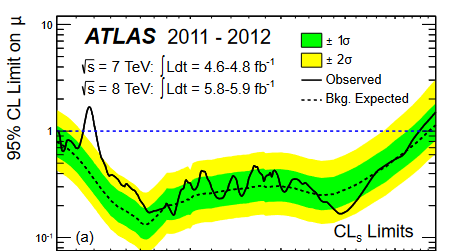
\includegraphics[width=0.6\textwidth]{pic/95CL.png}
    \caption{以 $m_H$ 为函数,展示了以信号强度参数 $\mu$ 表示的标准模型希格斯玻色子产生的置信度排除。}
    \label{fig:mH}
\end{figure}

\begin{itemize}
    \item 在 $95\%$ 置信度排除了从 \qty{110}{GeV} 到 \qty{582}{GeV} 的 $m_H$ 范围。
    \item 在 $99\%$ 置信度下,排除了三个质量区域,分别为 \qtyrange{113}{114}{GeV},\qtyrange{117}{121}{GeV} 和 \qty{132}{527}{GeV} 
\end{itemize}

在 $H\to ZZ(*)\to 4\ell$ 和 $H\to\gamma\gamma$ 通道中观察到了在 $m_H=\qty{126}{GeV}$ 附近的事件过剩,这两个通道都提供了具有高不变质量分辨率的完全重建候选事件。

\begin{figure}[htbp]
    \centering
    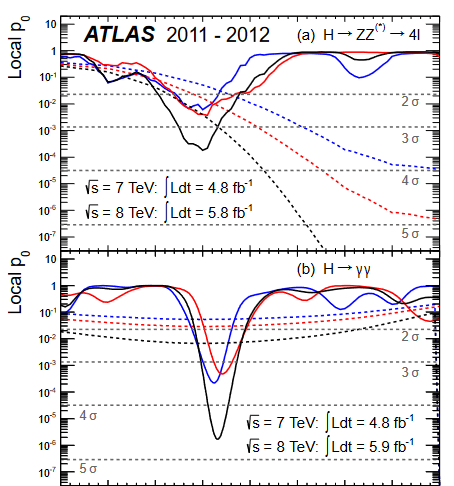
\includegraphics[width=0.6\textwidth]{pic/p0.png}
    \caption{.}
    \label{fig:p0}
\end{figure}

在 \qty{7}{TeV} 和 \qty{8}{TeV} 数据的组合中,最大的局部显著性发现在 SM 希格斯玻色子质量假设 $m_H=\qty{126.5}{GeV}$ 处,达到 $6.0\sigma$

这些结果提供了新粒子发现的确凿证据,其质量为 $\qty{126.0}{GeV} \pm 0.4(\text{统计}) \pm 0.4(\text{系统})$。对于以电荷和为零的矢量玻色子对的衰变,确认了新粒子为中性玻色子。
